\section{Compare the results of the first user journey}\label{section:results:comparison-first-journey}

This section explains the first user journey through the prototype and shows the three approaches' results. Figure \ref{fig:results:evaluation-first-path} shows the steps through the micro-frontend prototype used to measure the possible performance improvements of the shared caching layer and the reduction of queries. The client has to perform 13 steps throughout the prototype, which involves fetching almost every available GraphQL query. The dashboard micro-frontend yields some problems if the evaluation is started there. All widgets start to fetch their data simultaneously. Therefore, it can easily happen that multiple widgets fetch the same queries from the GraphQL \ac{API} because the data is not in the cache yet. This problem leads to a lot of theoretically unnecessary network requests and is difficult to circumvent. The evaluation shown in the figure is performed with an unauthenticated user. This section takes the measurements and compares the different approaches regarding request size, response size, the number of requests, and the total records fetched.

\ifshowImages
\begin{figure}[H]
  \centering
  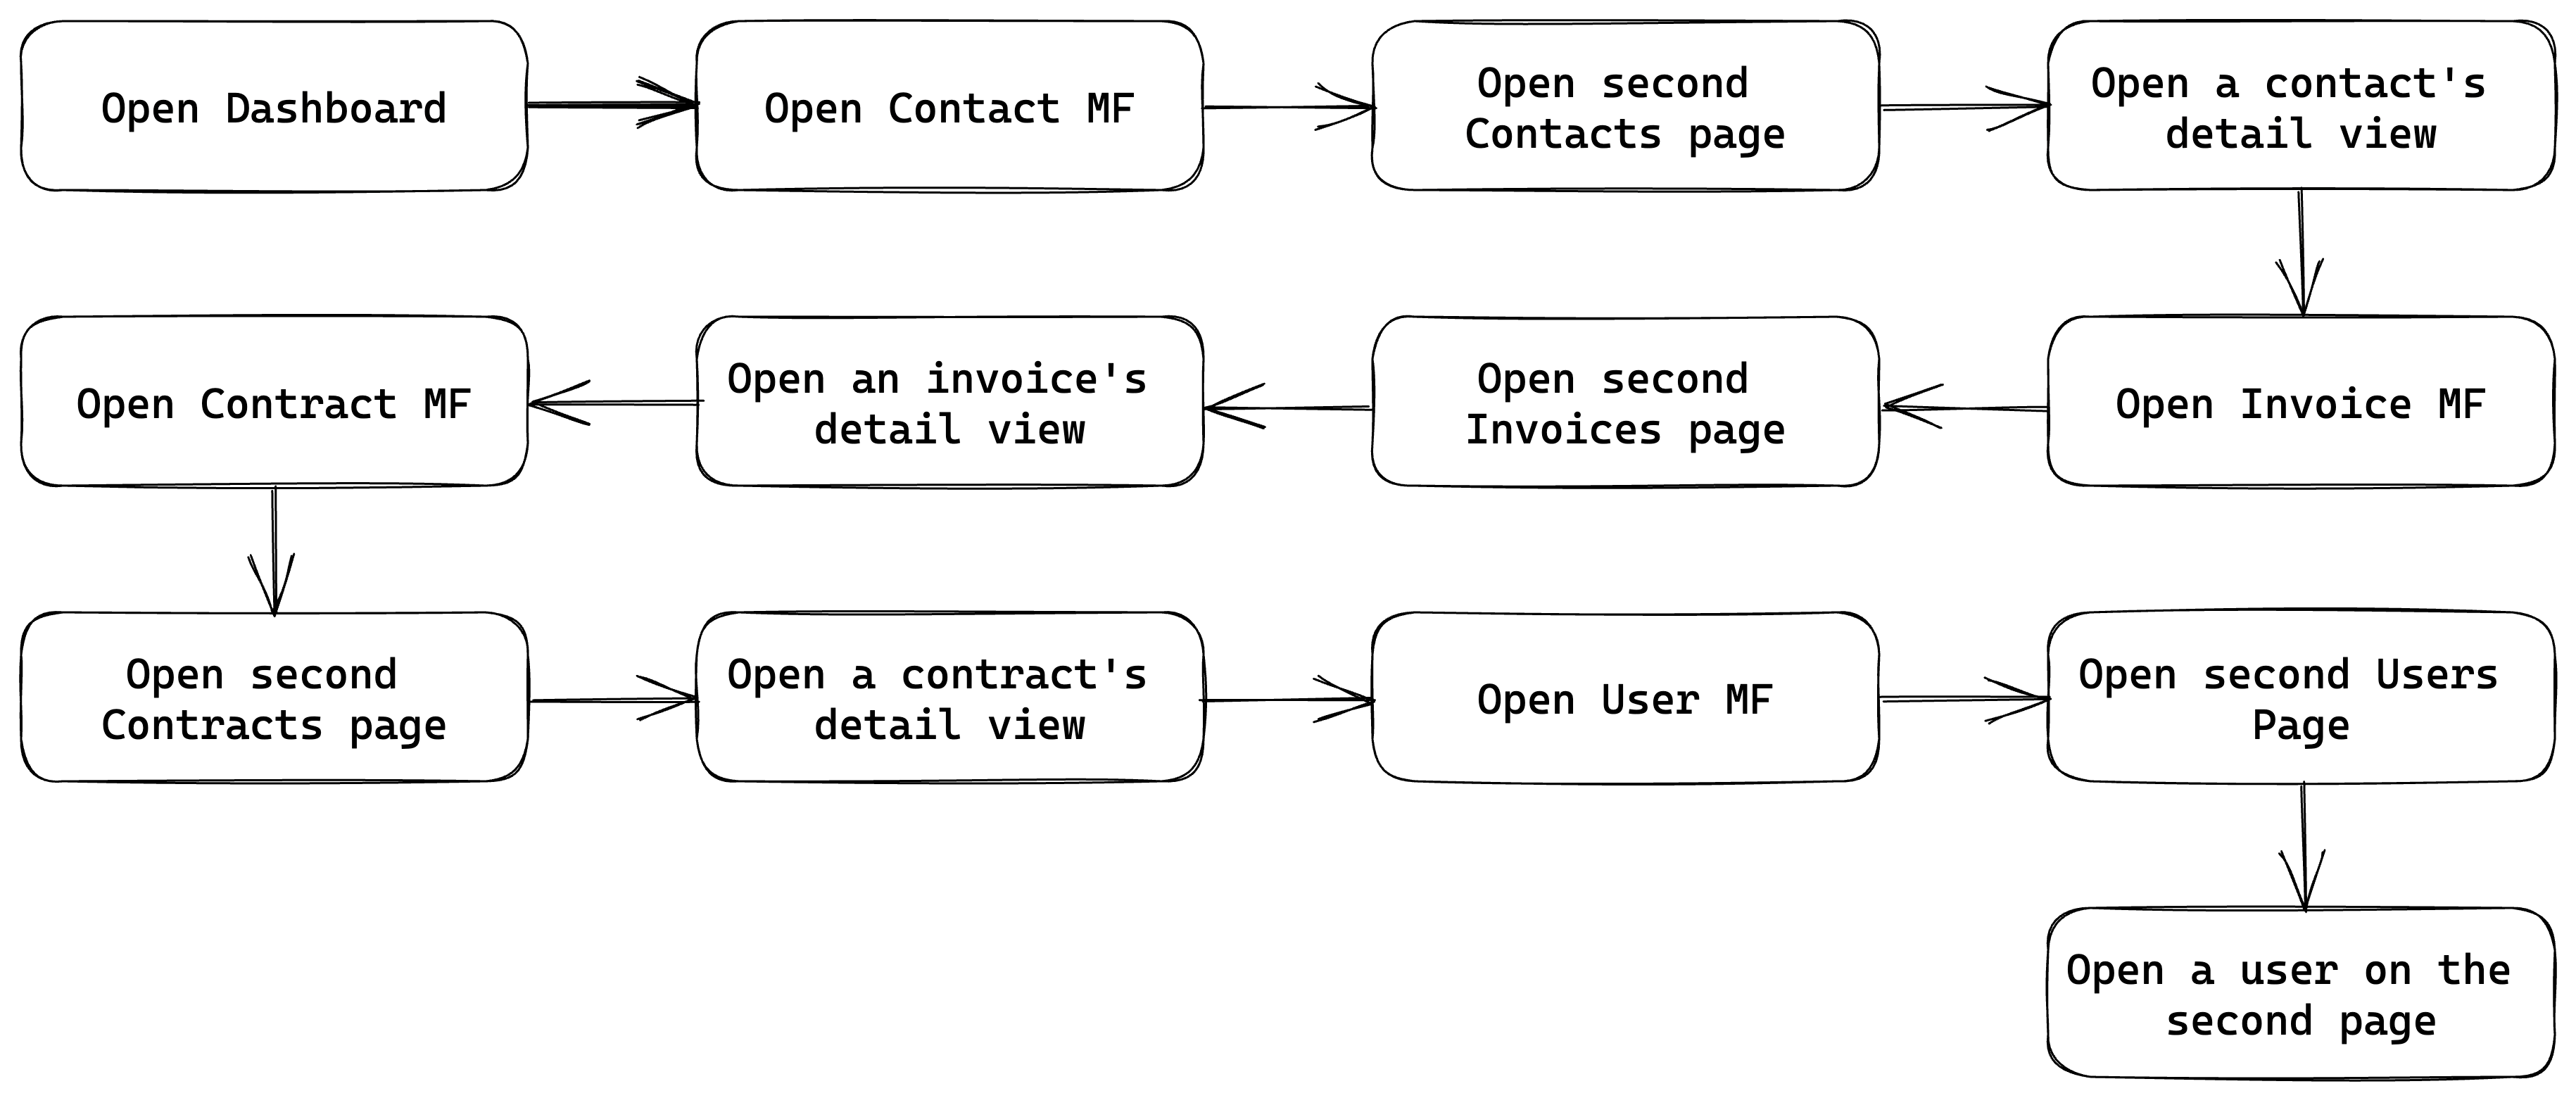
\includegraphics[width=1\linewidth]{images/results/evaluation-first-path.png}
  \caption{A user journey through the application to measure the performance of the micro-frontend architecture.}\label{fig:results:evaluation-first-path}
\end{figure}
\fi

\noindent Without a caching system, the GraphQL \ac{API} would have to execute 59 queries to provide the data for the user journey through the prototype. How to configure the prototype to use one of the three approaches has already been discussed in Section \ref{subsection:applied-methods:shared-caching-layer:graphql-client-creation} and Section \ref{subsection:applied-methods:query-reduction:testing-query-reduction}. The following sections describe and compare the results in more detail.

\subsubsection{Separate Cache and no reduced queries}\label{subsubsection:results:performance-measurement:separate-cache-no-reduction}

In this approach, each micro-frontend has its own instance of the Apollo Client and \texttt{InMemoryCache}. The queries were sent unaltered to the GraphQL \ac{API}. The following metrics were collected after the user journey was complete:

\begin{itemize}
  \item 47 network requests to the GraphQL \ac{API}
  \item 10.80 MB transferred (request size + response size)
\end{itemize}

\noindent The \texttt{GRAPHQL\_CLIENT\_OPTIONS\_CONFIG} and \texttt{REDUCE\_QUERY\_OPTIONS} injection tokens have to be configured the following way:

\begin{itemize}
  \item \texttt{shareCache: false}
  \item \texttt{reduceQueries: false}
\end{itemize}

\noindent A more detailed description of the configuration options can be found in Section \ref{subsection:applied-methods:shared-caching-layer:graphql-client-creation} and in Section \ref{subsection:applied-methods:query-reduction:testing-query-reduction}. 47 network requests have to be sent to the GraphQL \ac{API}, which can be seen in Figure \ref{fig:results:no-shared-cache-no-reduction}. The figure shows 54 requests, but 7 requests have to be subtracted because they are needed to make the integration of micro-frontends work. These requests fetch the micro-frontends and their settings from the remote location.

\ifshowImages
\begin{figure}[H]
  \centering
  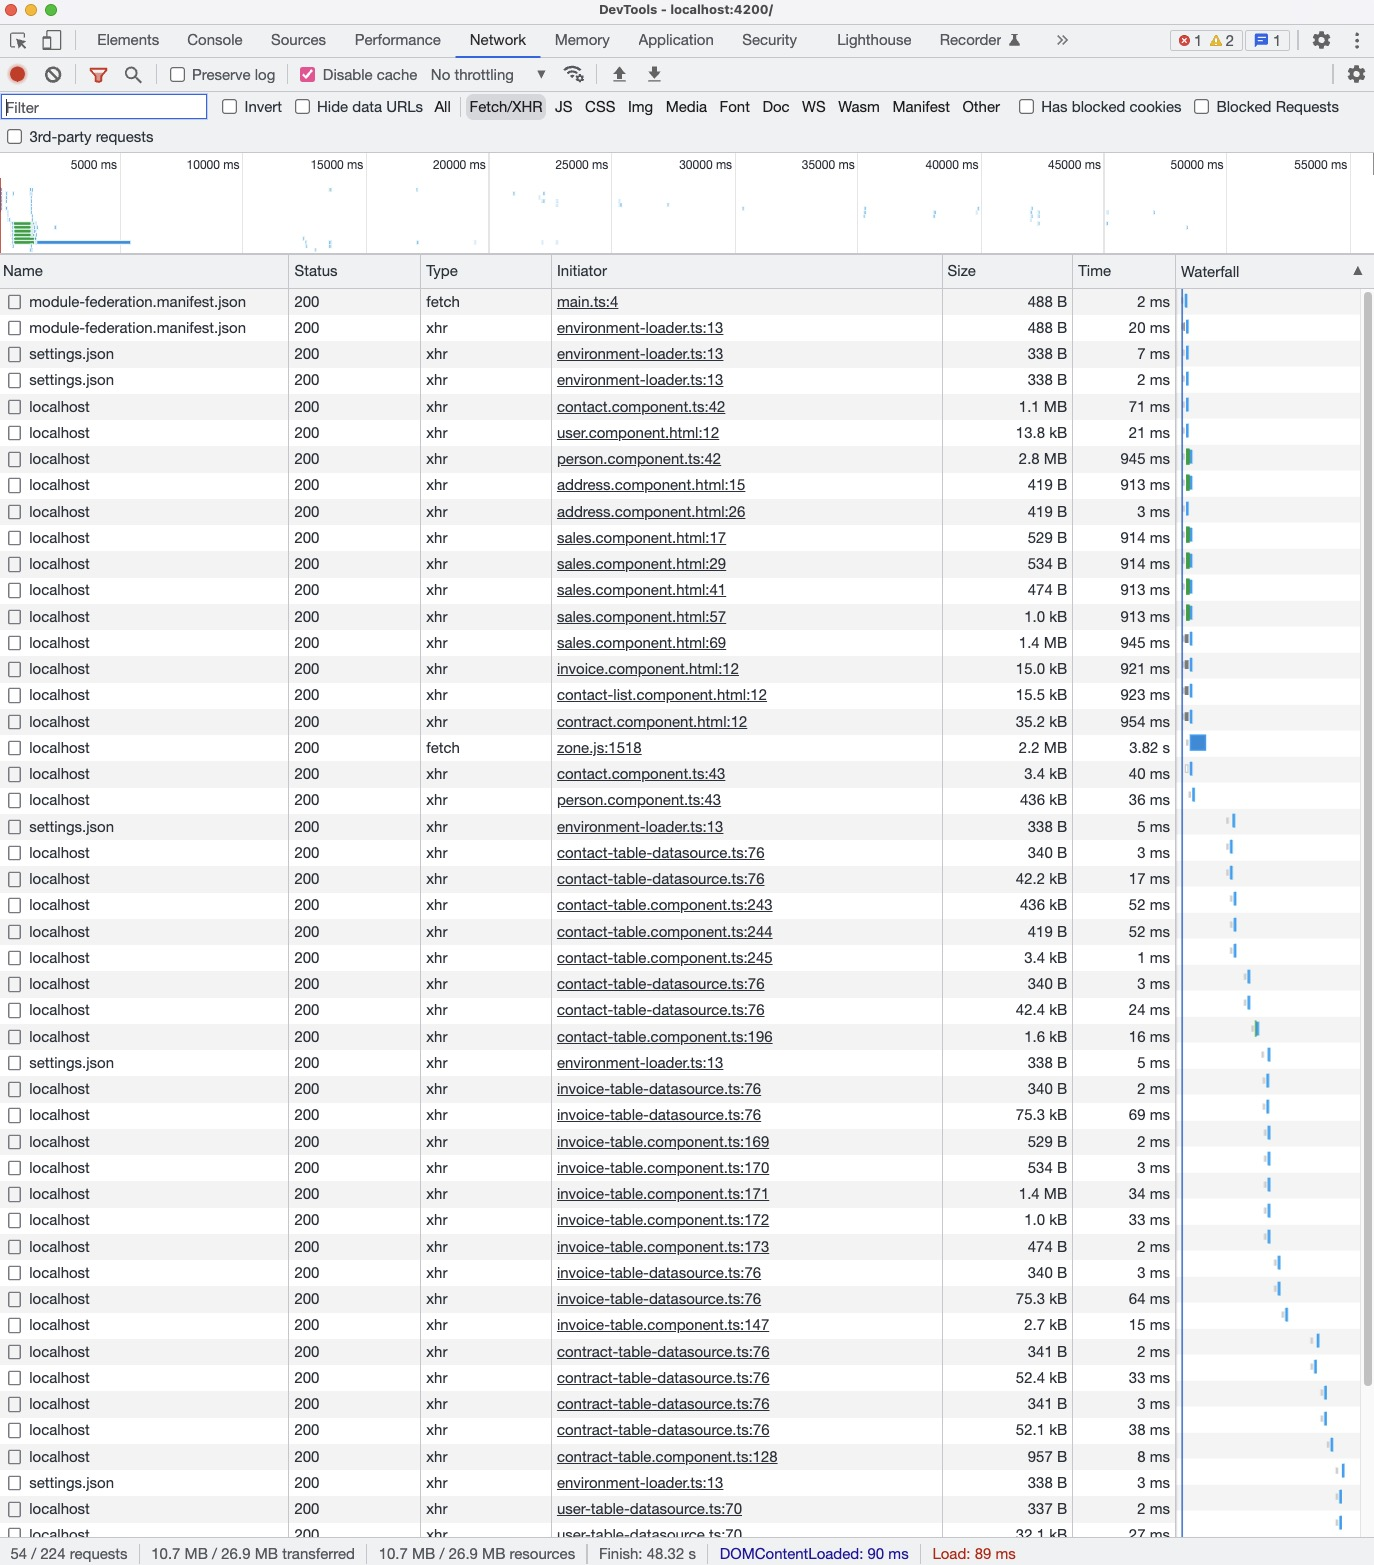
\includegraphics[width=0.8\linewidth]{images/results/1-attempt/no-shared-cache-no-reduction.jpg}
  \caption{Requests made during the measurement of the first approach.}\label{fig:results:no-shared-cache-no-reduction}
\end{figure}
\fi

\noindent The total size of the requests was 17.46 KB, and the responses were 10.78 MB. The 47 queries retrieve a total of 81510 records from the GraphQL  \ac{API}.

\subsubsection{Shared Cache and no reduced queries}\label{subsubsection:results:performance-measurement:shared-cache-no-reduction}

In this approach, a single cache instance is shared by all micro-frontends. The queries were sent unaltered to the GraphQL \ac{API}. The following metrics were collected after the user journey was complete:

\begin{itemize}
  \item 36 network requests to the GraphQL \ac{API}
  \item 8.45 MB transferred (request size + response size)
\end{itemize}

\noindent The \texttt{GRAPHQL\_CLIENT\_OPTIONS\_CONFIG} and \texttt{REDUCE\_QUERY\_OPTIONS} injection tokens have to be configured the following way:

\begin{itemize}
  \item \texttt{shareCache: true}
  \item \texttt{reduceQueries: false}
\end{itemize}

\noindent 36 requests have to be sent to the GraphQL \ac{API}, which can be seen in Figure \ref{fig:results:shared-cache-no-reduction}. Seven requests have to be deducted (\texttt{settings.json}, \texttt{module-federation.manifest.json}, \dots) as in the previous section.

\ifshowImages
\begin{figure}[H]
  \centering
  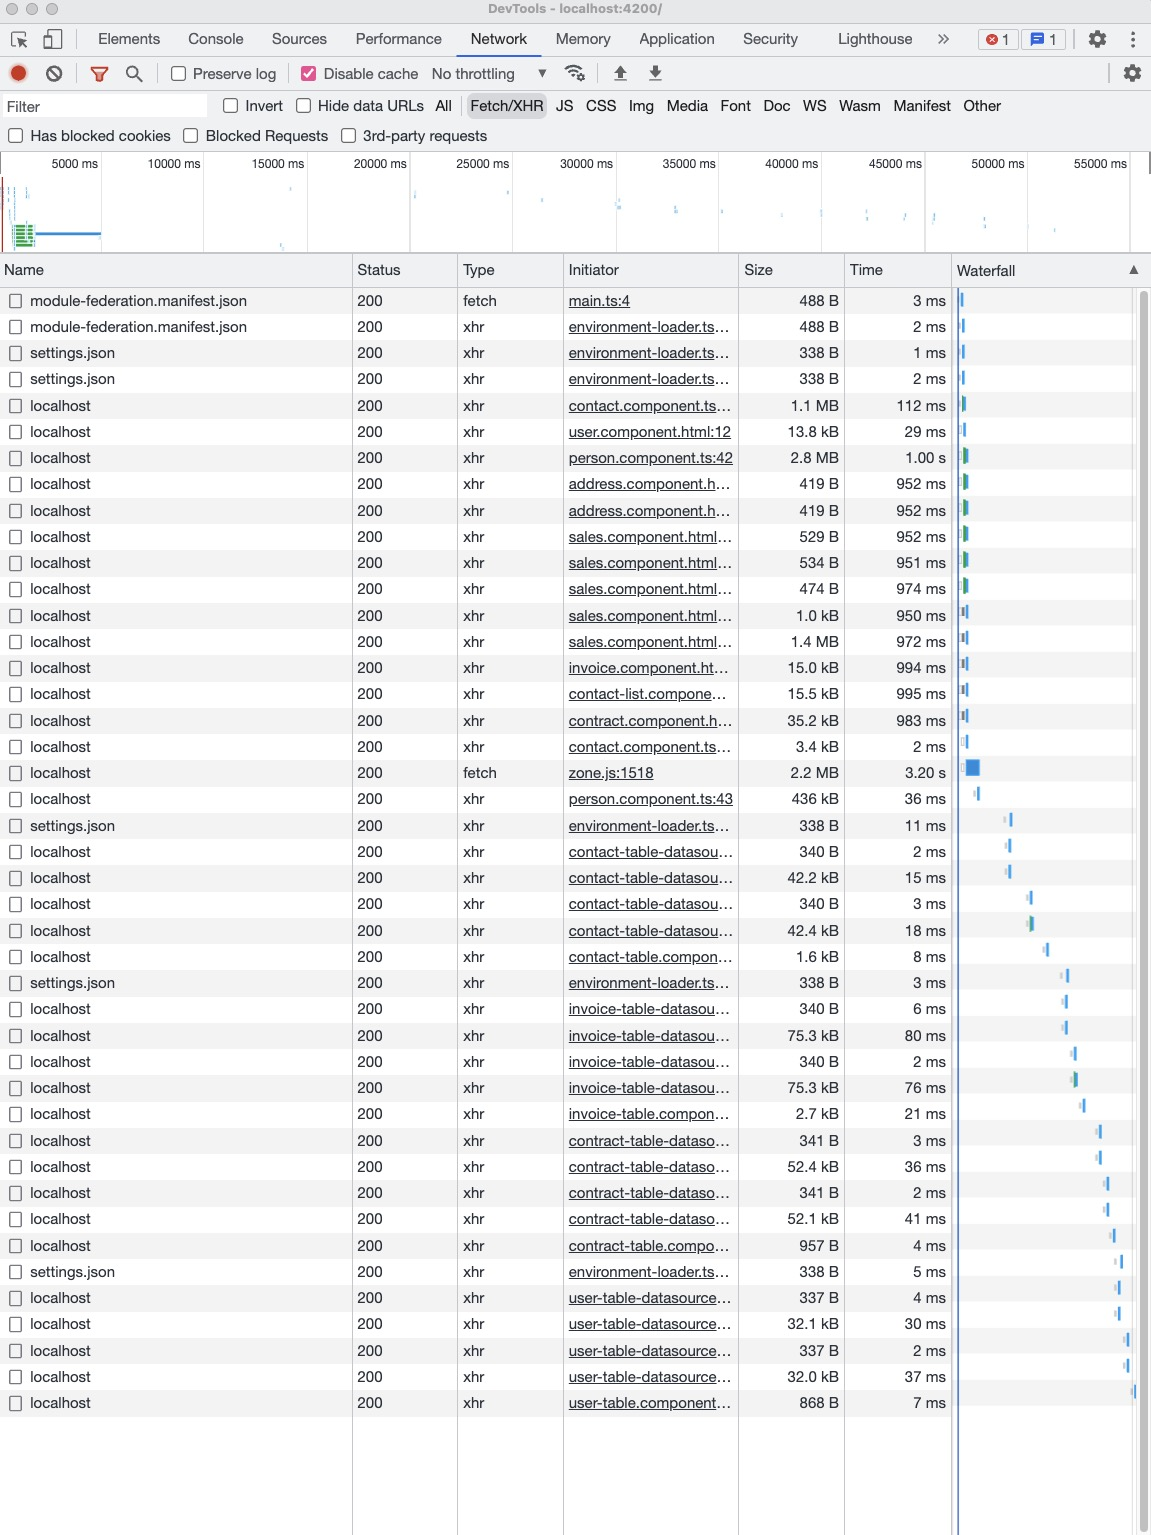
\includegraphics[width=0.8\linewidth]{images/results/1-attempt/shared-not-reduced-cache.jpg}
  \caption{Requests made during the measurement of the second approach.}\label{fig:results:shared-cache-no-reduction}
\end{figure}
\fi

\noindent The total size of the queries was 15.18 KB, and the size of the responses was 8.43 MB. The 36 queries retrieve a total of 51319 records from the GraphQL \ac{API}.

\subsubsection{Shared cache, query reduction}\label{subsubsection:results:performance-measurement:separate-cache-reduction}

In this approach, a single cache instance is shared between all micro-frontends. The queries are reduced by removing fields that are already inside the cache. The following metrics were collected after the user journey was complete:

\begin{itemize}
  \item 36 network requests to the GraphQL \ac{API}
  \item 8.39 MB transferred (request size + response size)
\end{itemize}

\noindent The \texttt{GRAPHQL\_CLIENT\_OPTIONS\_CONFIG} and \texttt{REDUCE\_QUERY\_OPTIONS} injection tokens have to be configured the following way:

\begin{itemize}
  \item \texttt{shareCache: true}
  \item \texttt{reduceQueries: true}
\end{itemize}

\noindent 36 requests have to be made to the GraphQL \ac{API}, which can be seen in Figure \ref{fig:results:shared-cache-reduction}. Seven requests have to be deducted (\texttt{settings.json}, \texttt{module-federation.manifest.json}, \dots) as in the previous sections.

\ifshowImages
\begin{figure}[H]
  \centering
  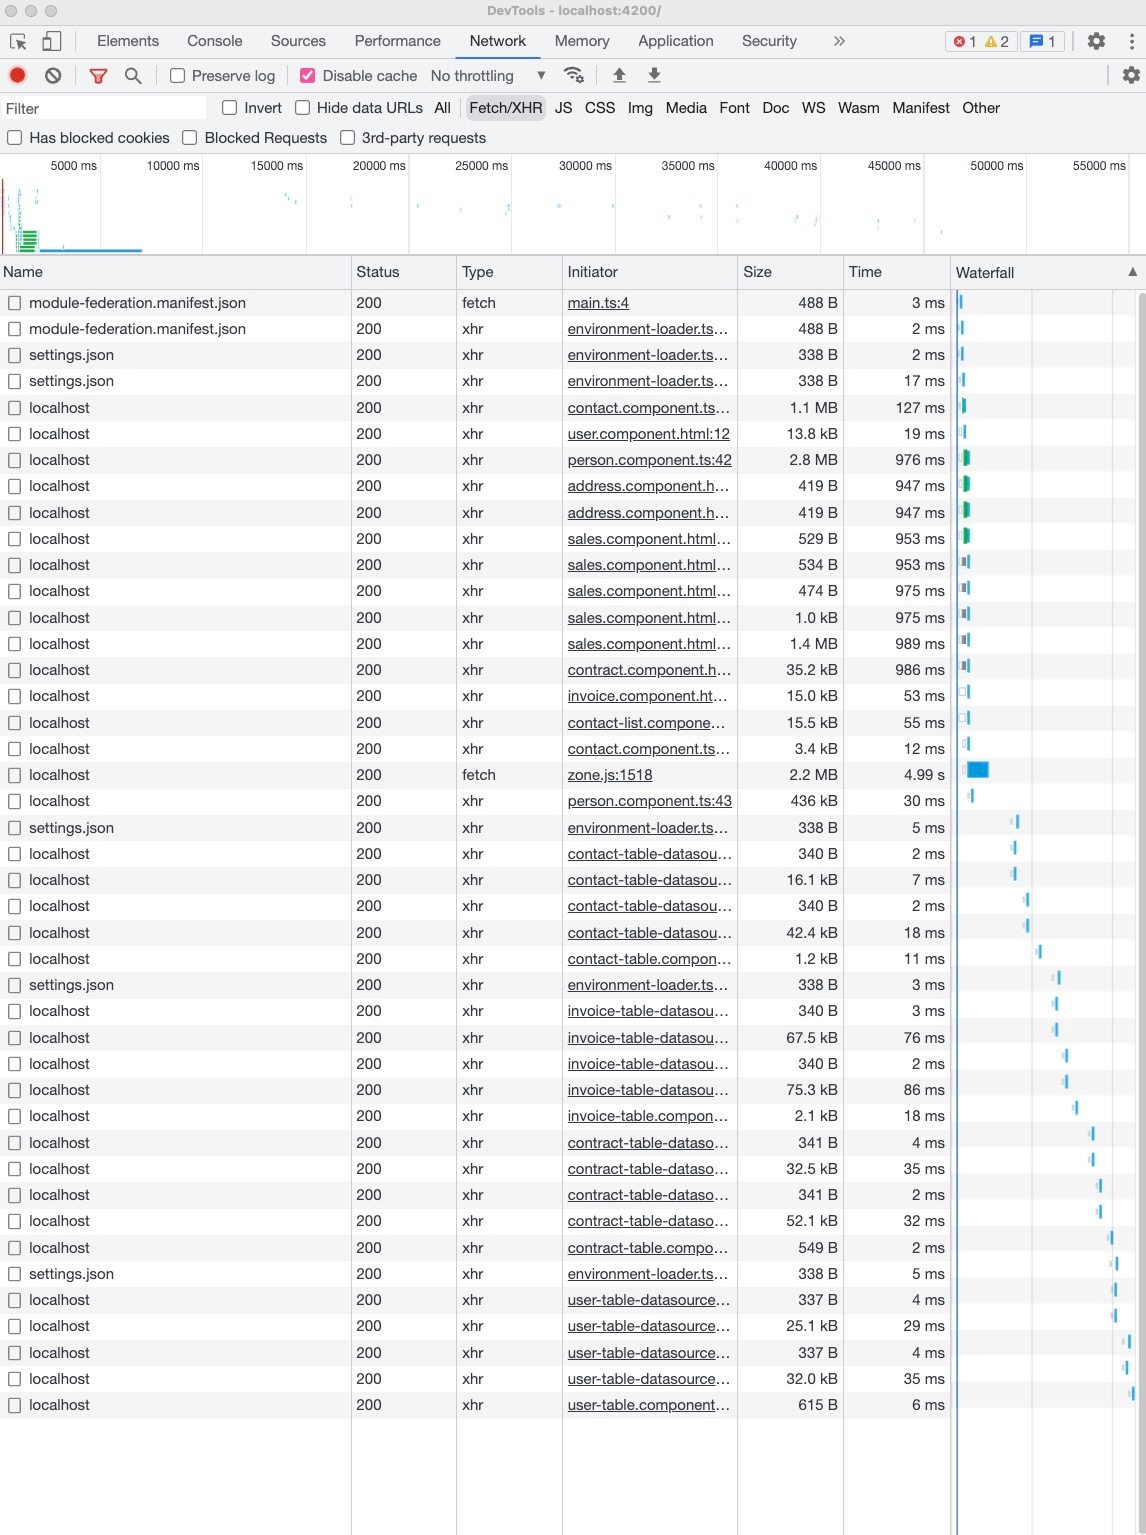
\includegraphics[width=0.8\linewidth]{images/results/1-attempt/shared-reduced-cache.jpg}
  \caption{Requests made during the measurement of the third approach.}\label{fig:results:shared-cache-reduction}
\end{figure}
\fi

\noindent The total size of the queries was 13.53 KB, and the size of the responses was 8.37 MB. The 36 queries retrieve a total of 51319 records from the GraphQL \ac{API}.

\subsection{Compare the first- and second-approach}\label{subsection:results:comparison-first-second-approach}

When comparing the first approach to the second, there is a significant difference in the number of network requests to the GraphQL \ac{API} and the size of the requests and responses, as seen in Table \ref{table:results:size-comparison-first-path-no-cache-no-reduction-cache-no-reduction}. The second approach requires 11 fewer network requests than the first approach. Since the queries are not altered for this comparison, the additional network requests are responsible for the overall difference in request- and response size. The 11 additional requests from the first approach send an additional 2.29 KB to the \ac{API} and return about an additional 2.34 MB from the \ac{API}. Therefore, 22\% of the total response size can be saved using a shared caching layer for all micro-frontends. Another interesting observation is that the shared cache approach retrieves 30191 fewer records than the naive approach, about 37\% of the total records returned. Many queries need to be retrieved more than once in the first approach, hence the large difference in the number of records.

\ifshowTables
\begin{table}[H]
  \begin{tabular}{|l|l|l|l|l|}
  \hline
    & \textbf{Req. Size (B)} & \textbf{Resp. Size (B)} & \textbf{Requests} & \textbf{Records} \\
    \hline
    \textbf{No Reduction, Separate Cache} & 17462 & 10780656 & 47 & 81510 \\
    \hline
    \textbf{No Reduction, Shared Cache} & 15176 & 8437211 & 36 & 51319 \\
    \hline
    \hline
    \textbf{Diff (B)} & \textbf{2286} & \textbf{2343445} & \textbf{11} & \textbf{30191} \\
    \hline
    \textbf{Reduction (\%)} & \textbf{13\%} & \textbf{22\%} & \textbf{23\%} & \textbf{37\%} \\
    \hline
  \end{tabular}
  \caption{First Journey: Compare the requests and responses of the first- and second-approach.}\label{table:results:size-comparison-first-path-no-cache-no-reduction-cache-no-reduction}
\end{table}
\fi

\noindent The following enumeration shows which and how often a GraphQL query was discarded when using a shared caching layer between the micro-frontends compared to a separate cache:

\begin{itemize}
  \item allCountries: 2
  \item allSalutations: 2
  \item allTitles: 2
  \item allArticleUnits: 1
  \item allCurrencies: 1
  \item allVats: 1
  \item allSalesCountries: 1
  \item allInvoiceTypes: 1
\end{itemize}

\noindent The data from the omitted requests is typically used for populate selection controls within detail views and has to be retrieved repeatedly in each micro-frontend. The first three queries are used for widgets on the dashboard, the Contact application, and the User application. The last five queries are used for Dashboard widgets and the Sales application.

\subsection{Compare the first- and third-approach}\label{subsection:results:comparison-first-third-approach}

As in the previous comparison, there is the same difference in the number of network requests made to the GraphQL \ac{API}. As before, there is a massive difference in the size of the responses and the requests. The results are shown in Table \ref{table:results:size-comparison-first-path-no-cache-no-reduction-cache-reduction}. Just as before, there is a difference of 11 GraphQL queries that are sent to the GraphQL \ac{API}. However, due to the reduction of queries, the difference in the size of the requests and responses is greater than in Section \ref{subsection:results:comparison-first-second-approach}. All queries of the first approach send 3.93 KB more and return about 2.41 MB more from the GraphQL \ac{API} compared to the third approach. A shared cache and query reduction can save about 22\% response sizes. As before, 37\% fewer records need to be retrieved from the GraphQL \ac{API}.

\ifshowTables
\begin{table}[H]
  \begin{tabular}{|l|l|l|l|l|}
  \hline
  & \textbf{Req. size (B)} & \textbf{Resp. size (B)} & \textbf{Requests} & \textbf{Records}  \\
  \hline
  \textbf{No Reduction, Separate Cache} & 17462 & 10780656 & 47 & 81510 \\
  \hline
  \textbf{Reduction, Shared Cache} & 13533 & 8374763 & 36 & 51319 \\
  \hline
  \hline
  \textbf{Diff (B)} & \textbf{3929} & \textbf{2405893} & \textbf{11} & \textbf{30191} \\
  \hline
  \textbf{Reduction (\%)} & \textbf{23\%} & \textbf{22\%} & \textbf{23\%} & \textbf{37\%} \\
  \hline
  \end{tabular}
  \caption{First Journey: Compare the requests and responses of the first- and third-approach.}\label{table:results:size-comparison-first-path-no-cache-no-reduction-cache-reduction}
\end{table}
\fi

\subsection{Compare the second- and third-approach}\label{subsection:results:comparison-second-third-approach}

Between the second and third approaches, there is almost no difference in request- and response size compared to the comparisons from Sections \ref{subsection:results:comparison-first-second-approach} and \ref{subsection:results:comparison-first-third-approach}, as seen in Table \ref{table:results:size-comparison-first-path-cache-no-reduction-cache-reduction}. Both approaches have the same number of queries sent to the GraphQL \ac{API} since all micro-frontends use the same cache instance. Removing fields from queries does not lead to fewer network requests, because it just removes fields from queries. Network requests would only be omitted if all of the data is already in the cache, but then the query would not be reduced. The difference in request and response size between the two approaches comes solely from query reduction. Using the third approach, the difference in request size is about 1.64 KB (11\%), which is insignificant. The difference between the response sizes (62.45 KB) is almost zero relative to the amount of data returned.

\ifshowTables
\begin{table}[H]
  \begin{tabular}{|l|l|l|l|l|}
  \hline
  & \textbf{Req. size (B)} & \textbf{Resp. size (B)} & \textbf{Requests} & \textbf{Records} \\
  \hline
  \textbf{No Reduction, Shared Cache} & 15176 &  8437211 & 36 & 51319 \\
  \hline
  \textbf{Reduction, Shared Cache} &  13533 &  8374763 & 36 & 51319 \\
  \hline
  \hline
  \textbf{Diff (B)} & \textbf{1643} & \textbf{62448} & \textbf{0} & \textbf{0} \\
  \hline
  \textbf{Reduction (\%)} & \textbf{11\%} & \textbf{1\%} & \textbf{-} & \textbf{-} \\
  \hline
  \end{tabular}
  \caption{First Journey: Compare the requests and responses of the second- and third-approach.}\label{table:results:size-comparison-first-path-cache-no-reduction-cache-reduction}
\end{table}
\fi